\documentclass[11pt]{article}
\usepackage[margin = 1in]{geometry}
\usepackage{amsmath}
\usepackage{amssymb}
\usepackage{amsthm} % for proof environment
\usepackage{enumitem}
\usepackage{graphicx}
\usepackage{indentfirst}
\usepackage{caption}
\usepackage{lscape}
\usepackage{multirow}
\usepackage{array}
\usepackage{setspace}
\setlist{nolistsep}
\usepackage[round]{natbib}
\usepackage{accents}

\newcommand{\ubar}[1]{\underaccent{\bar}{#1}}
\newcommand{\p}{\prime}
\newcommand{\ev}{\mathbb{E}}
\newcommand{\lagr}{\mathcal{L}}
\newcommand{\inv}[1]{#1^{-1}}
\newcommand{\R}{{\rm I\!R}}
\newcommand{\U}{\mathcal{U}}
\renewcommand{\H}{\mathcal{H}}
\newcommand{\pderiv}[2]{\frac{\partial#1}{\partial #2}}

\begin{document}
    \begin{flushleft}
        Optimal Taxation with Heterogeneous Rates of Return \\
        Two-Type Case \\
        \today
    \end{flushleft}

\section{Two-Type Case}
\subsection{Immobile Capital} \label{t2_imm}
Here, I consider a model in which households are one of two types \( \theta\in\{\theta_L, \theta_h\} \) with \( \Pr(\theta = \theta_H) = \pi \). The social planner solves the usual problem:
\begin{align}
    \max &\sum_{i \in\{L,H\}}\left[ u(w - k(\theta_i)) + \beta u(c(\theta)) \right]\pi_i \\ 
    &\text{s.t.} \notag \\
    &\sum_{i \in\{L,H\}}\left[ \theta_i k(\theta_i) - c(\theta_i) \right]\pi_i \ge E \\
    &u(w - k(\theta_H)) + \beta u(c(\theta_H)) \ge u\left( w - \frac{\theta_L}{\theta_H}k(\theta_L) \right) + \beta u(c(\theta_L)) \label{ic_H} \\
    &u(w - k(\theta_L)) + \beta u(c(\theta_L)) \ge u\left( w - \frac{\theta_H}{\theta_L}k(\theta_H) \right) + \beta u(c(\theta_H)) 
\end{align}

I use the following parametrization:
\begin{align*}
    \beta &= 0.95 & w &= 1.2\\
    E &= 0 & \pi &= 0.3
\end{align*}

In general, the planner requires that households of type \( \theta_L \) invest in the first period. This level of investment can be low, particularly if \( \theta_L \) is far below 1 and \( \theta_H \) is large in relation to \( \theta_L \). However, it does seem that for most specifications, the planner finds it optimal to have \( k(\theta_L) > 0 \), likely due in part to satisfy the incentive constraint for the high type (\ref{ic_H}). Figure \ref{fig_imm} shows the optimal levels of investment for the high and low types, for two different values of \( \theta_L \), and on the \( x \)-axis the ratio of \( \theta_H \) to \( \theta_L \).
%
\begin{figure}[!ht]
    \centering
    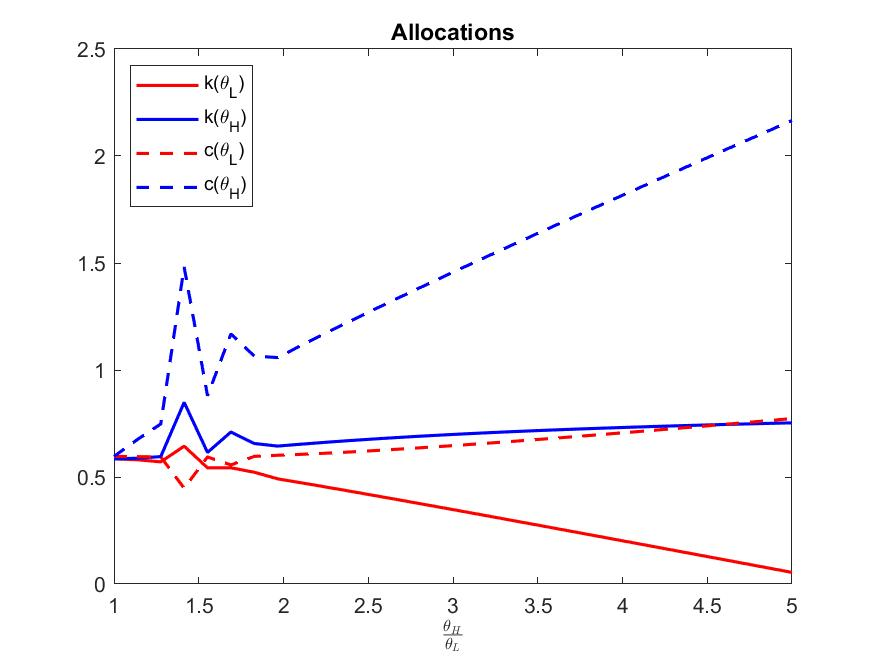
\includegraphics[scale = 0.5]{figures/immob.jpg}
    \caption{Optimal Investment. The solid lines show \( k(\theta_L) \), and the dashed lines \( k(\theta_H) \).}
    \label{fig_imm}
\end{figure}

\subsection{Mobile Capital} \label{t2_mob}

Here I consider the same model as in section \ref{t2_imm}, but allow for the borrowing and lending of risk-free bonds \( b \) between the households in the first period. Thus, the planner's problem becomes

\begin{align}
    \max &\sum_{i \in\{L,H\}}\left[ u(w - k(\theta_i) - b(\theta_i)) + \beta u(c(\theta)) \right]\pi_i \\ 
    &\text{s.t.} \notag \\
    &\sum_{i \in\{L,H\}}\left[ \theta_i k(\theta_i) - c(\theta_i) \right]\pi_i \ge E \\
    &u(w - k(\theta_H) - b(\theta_H)) + \beta u(c(\theta_H)) \ge u\left( w - \frac{\theta_L}{\theta_H}k(\theta_L) - b(\theta_L)\right) + \beta u(c(\theta_L)) \\
    &u(w - k(\theta_L) - b(\theta_L)) + \beta u(c(\theta_L)) \ge u\left( w - \frac{\theta_H}{\theta_L}k(\theta_H) - b(\theta_H) \right) + \beta u(c(\theta_H)) 
\end{align}

Aside from the allowance for borrowing and lending, the model is the same as in section \ref{t2_imm}. In this case, if \( \theta_H \) is sufficiently large relative to \( \theta_L \), then \( k(\theta_L) = 0 \). The optimal borrowing and lending allocations call for \( \theta_H \) types to be net borrowers in the first period, allowing them to invest more, and for \( \theta_L \) types to be net lenders. Figure \ref{fig_mob} show the optimal investment \( k \) and lending \( b \) for each type, as in Figure \ref{fig_imm}. 

\begin{figure}[!ht]
    \centering
    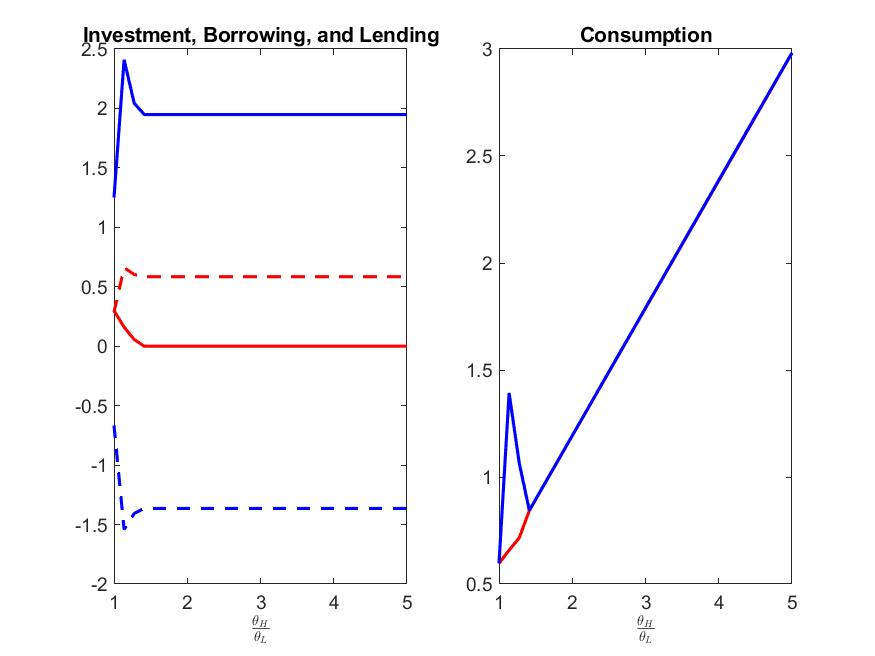
\includegraphics[scale = 0.5]{figures/mob.jpg}
    \caption{Optimal Investment and Lending. The dashed lines show the allocations for \( \theta_H \), and the solid lines \( \theta_L \).}
    \label{fig_mob}
\end{figure}

\end{document}